%% Pattern Recognition Letters version of the manuscript (generated by build_prl_tex.py; numbers come from results/*.json)
\documentclass[final,5p,times,twocolumn,authoryear]{elsarticle}
\IfFileExists{prletter.sty}{\usepackage{prletter}}{}
\usepackage{amsmath,amssymb}
\usepackage{graphicx}
\usepackage{booktabs}
\usepackage[T1]{fontenc}
\usepackage{url}
\journal{Pattern Recognition Letters}
\biboptions{authoryear}

\begin{document}
\begin{frontmatter}

\title{Rarity and local order: two complementary label-free channels for anomaly detection on lattices of embeddings}

\author[a]{Leon Sandler\corref{cor1}}
\cortext[cor1]{Corresponding author. e-mail: sandler.leon@gmail.com; ORCID 0009-0007-4584-808X}
\address[a]{Independent Researcher, Northbrook, IL, USA}

\begin{abstract}
Anomaly scores on lattices of embeddings, such as image patches, usually measure how rare the embedding of a site is. We show on simulated data that rarity is one of two complementary label-free channels. Channel A is the rarity aggregated with weights given by the similarity of neighboring embeddings; it preserved scattered and bar-shaped anomalies that a fixed $3\times3$ mean destroyed (lower-tail average precision 0.32 against 0.11 on ten independent test scenarios), and a contrast-survival model explains the loss. Channel B is a directional form of the local disorder of the MyUncle lattice model, the minimum of the disorder over the four quadrants of a site. It detects arrangement anomalies, the same embeddings in the wrong places: there the rarity stayed at chance (average precision 0.06) and channel B reached 0.86. A label-free tail index chooses the channel per cohort; on fifteen independent test scenarios this raised the lower-tail average precision from 0.20 to 0.36 (paired 95\% interval of the gain +0.10 to +0.25) without loss on the scenarios with feature anomalies only. Order gates and an evolutionary configuration search did not help, and cohorts with both kinds of anomaly need both maps. Code and results are open.
\end{abstract}

\begin{keyword}
anomaly detection \sep embedding lattices \sep spatial arrangement \sep orientational order \sep similarity-weighted aggregation \sep label-free fusion
\end{keyword}

\end{frontmatter}

\section{Introduction}
Many pattern recognition problems put a vector on every site of a grid: the embeddings of the patches of an image, or the orientation field of an ordered medium. Unsupervised anomaly detection on such lattices usually asks how rare the embedding of a site is, for example by its distance to the nearest members of a memory of normal embeddings \citep{Roth2022}; it has been developed for surveys in astronomy \citep{Baron2017,Lochner2021} and for medical images \citep{Schlegl2019}. Two things are rarely measured. First, the per-site scores are routinely smoothed over a fixed window, and the failure modes of that step are not reported. Second, a rarity score, however it is aggregated, sees only \emph{what} is at a site. An anomaly that consists of ordinary elements in the wrong arrangement, a contextual anomaly \citep{Chandola2009} or, in industrial inspection, a logical anomaly \citep{Bergmann2022}, leaves the distribution of the embeddings unchanged.

MyUncle \citep{MyUncle2026} is a simulation framework for a maintenance lattice (rotors whose order is eroded by a state-dependent flux and restored by repair); its central quantity is the local order of the unit vectors on neighboring sites. This paper shows that this quantity, in a directional form, supplies the second channel that rarity lacks. Contributions: (1) \emph{channel A}: rarity aggregated with weights given by the similarity of neighboring embeddings, which preserved the anomalies that a fixed window destroyed, and a contrast-survival model that explains the loss; (2) \emph{channel B}: the directional local disorder, which detects arrangement anomalies to which rarity is blind and, unlike the isotropic disorder and the distance of a site to its neighbors, does not respond to walls between ordered domains; (3) a label-free tail index that selects the channel per cohort, evaluated once on fifteen independent test scenarios with paired confidence intervals; (4) what did not help: gates on local order and on the von Mises--Fisher information, a nucleation-and-growth rule, and a search with GaaR \citep{GaaR2026}, an evolutionary search framework, which did not beat random search; and (5) an open pipeline \citep{MyUncleVision2026}. All evidence is simulated; no experimental image was analyzed.

\section{Scores}
\subsection{Rarity}
Each site $i$ carries a unit vector $u_i$. For images, a patch is a $224\times224$ px window (0.5~$\mu$m/px) encoded by DINOv2 ViT-S/14 \citep{Oquab2023} (384-d, pretrained on natural images) or by a deterministic handcrafted encoder of color, gradient-orientation and texture statistics (64-d; \citealp{Ruifrok2001}); embeddings are centered, reduced by a cohort PCA (16 components; \citealp{Pedregosa2011}) and normalized. For simulated lattices the vector is the rotor $(\cos\theta,\sin\theta)$, optionally with the local disorder as a third coordinate; the intact flag is never part of it. The rarity $r_i$ is the cohort percentile of the mean cosine distance to the $k$ nearest sites of a reference sample (same-image neighbors within six steps excluded), evaluated with $k$ equal to 0.5, 1, 2, 5 and 10\% of the sample, the highest rank counting, because the prevalence of an interesting state is not known in advance.

\subsection{Channel A: aggregation of the rarity}
A rule turns $r$ into a score $s$ using the lattice neighbors in a $w\times w$ window $W_i$ and the unit embeddings, never labels. The frozen configuration of earlier versions of this work is the fixed mean, $s_i=|W_i|^{-1}\sum_{j\in W_i}r_j$ with $w=3$. Similarity-weighted aggregation weights each neighbor by the compatibility of its embedding with that of site $i$,
\begin{equation}
c_{ij}=\exp\!\bigl(-(1-u_i^{\top}u_j)/\tau\bigr),\qquad s_i=\frac{\sum_{j\in W_i}c_{ij}\,r_j}{\sum_{j\in W_i}c_{ij}},
\end{equation}
with $\tau$ the median of $1-u_i^\top u_j$ over lattice-adjacent pairs of the cohort (label-free, no free parameter). It is an edge-preserving filter in embedding space of the bilateral kind; we make no claim to its novelty. Further rules were tested and are reported in Section~\ref{sec:neg}: gates that mix the unsmoothed and the aggregated score, $s_i=(1-g_i)r_i+g_i\,s^{\mathrm{sim}}_i$ with $g_i=\sigma(\alpha(A_i-\vartheta))$ and $A_i$ the cohort rank of the mean compatibility, of the resultant length $R_i$ or of the von Mises--Fisher order information $H_\chi$ of the neighbors; a one-sided rule that lets neighbors add evidence but never remove it; a nucleation-and-growth rule with hysteresis, in which a site above a nucleation threshold seeds and raises weaker compatible neighbors \citep{Canny1986}; and a persistence factor over the windows 1, 3, 5, 7.

\subsection{Local order and entropy}
MyUncle's local disorder is $D_i=1-R_i$ with $R_i=\bigl|\tfrac{1}{|N_i|}\sum_{j\in N_i}u_j\bigr|$ over the four neighbors $N_i$, valid in any dimension. The concentration $\kappa_i$ of the von Mises--Fisher distribution on $S^{d-1}$ \citep{Banerjee2005,Mardia2000} with mean resultant length $R_i$ solves $A_d(\kappa)=I_{d/2}(\kappa)/I_{d/2-1}(\kappa)=R_i$, and the information held in the local order is $H_\chi=S_{\mathrm{unif}}-S_{\mathrm{vMF}}(\kappa,d)$ with
\begin{equation}
S_{\mathrm{vMF}}=-\bigl(\tfrac d2-1\bigr)\ln\kappa+\tfrac d2\ln(2\pi)+\ln I_{d/2-1}(\kappa)-\kappa A_d(\kappa).
\end{equation}
For $d=2$ these are MyUncle's quantities; the tests agree with the unmodified core to $10^{-12}$ (disorder) and $10^{-9}$ (entropy; Fig.~\ref{fig:bridge}). $H_\chi$ is a monotone function of $R_i$, so every statement below about the rank of the disorder holds for the rank of $H_\chi$.

\begin{figure}[t]
\centering
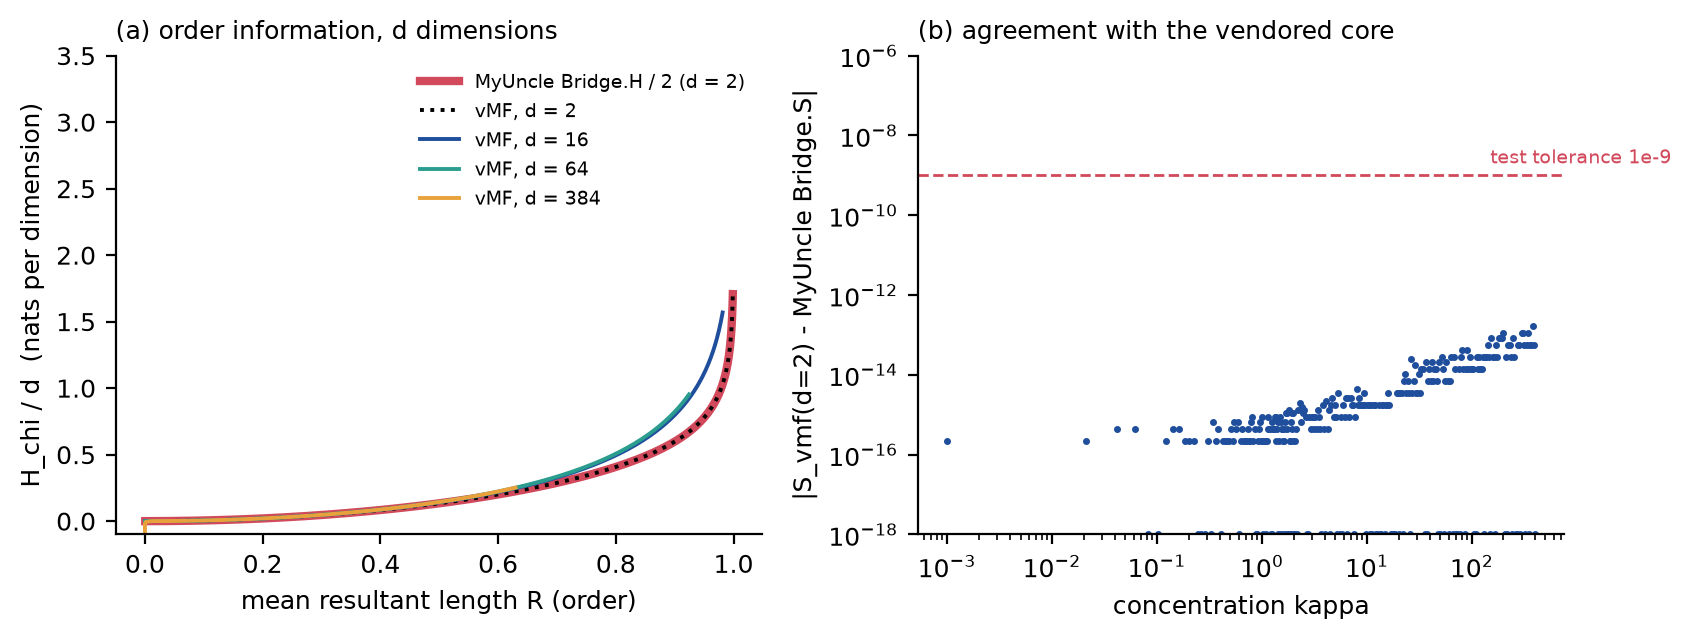
\includegraphics[width=0.95\columnwidth]{fig_bridge.png}
\caption{(a) The order-information bridge in $d$ dimensions: MyUncle's $H_\chi$ ($d=2$, red) and the von Mises--Fisher generalization for $d=2$, 16, 64 and 384. (b) Difference between the $d=2$ entropy and the vendored MyUncle function.}
\label{fig:bridge}
\end{figure}

\subsection{Channel B: directional disorder, and the choice of the channel}
The isotropic disorder $D_i$ is large wherever neighboring vectors differ, which includes every wall between two ordered domains. Let $Q_i^1,\dots,Q_i^4$ be the four $2\times2$ quadrant windows that contain site $i$. The directional disorder is
\begin{equation}
B_i=\min_{q}\Bigl(1-\Bigl|\tfrac14\sum_{j\in Q_i^q}u_j\Bigr|\Bigr).
\end{equation}
A wall is ordered on at least one side, so one quadrant lies inside one domain and $B_i$ stays near zero, while a disorganized region is disordered in every direction. Taking the minimum over sub-windows is the idea of the edge-preserving filter of \citet{Kuwahara1976}, applied here to the order parameter instead of the variance; quadrants with a missing site do not count.

The two channels have different units, so they are compared through a label-free \emph{tail index}: the raw score of a channel (the nearest-neighbor distance at $k=1\%$ for channel A, $B_i$ for channel B) is standardized over the cohort with the median and the median absolute deviation \citep{Rousseeuw1993}, and the tail index $T$ is the 97th percentile of the result (1.88 for a Gaussian bulk without anomalies). The fused detector uses channel B for a cohort when $T_B>T_A$ and $T_B>2\times1.88$, and channel A, the similarity-weighted rarity, otherwise. The choice is made once per cohort and uses no labels. Site-wise alternatives were evaluated as well: the maximum of the two standardized scores, the maximum of the two cohort ranks, and a maximum of the ranks weighted by $T^p$ ($p=1,2,4$).

\section{Evaluation design}
\textbf{Scenarios.} (i) Synthetic stained-tissue images ($4480\times4480$ px; tubule-like rings, glomerulus-like discs, vessels, stain variation, planted anomalies and artifacts; 8 development and 16 held-out images, the latter with three anomaly types not used in development), each with the handcrafted and the DINOv2 embedding. (ii) Lattices simulated with MyUncle's kinetic Monte Carlo (unmodified core; $48\times48$ sites, snapshots at steps 20, 40, 60, damaged sites as ground truth), with the rotor and rotor + $D$ embeddings; the development preset is chiral scaffold, the test presets are superconducting scaffold, polymer photodegradation, liquid crystal and magnetic storage decay, which are model parameter sets, not fitted to measurements. (iii) A controlled generator of embedding lattices ($32\times32$ sites, 16 dimensions, piecewise-constant background domains, 3\% anomalous sites of fixed separability, 10 images per cohort, 5 cohorts) in which only the shape of the \emph{feature outliers} changes: scattered single sites, $3\times3$ and $6\times6$ blocks, bars of 8 sites, irregular 12-site clusters, and $3\times3$ blocks on domain boundaries; each anomaly has its own direction. (iv) \emph{Arrangement anomalies}: a spatially correlated background (a smooth random field) in which the embeddings of a region are permuted among its sites, so that every embedding keeps its value and only the arrangement is destroyed ($6\times6$ and $8\times8$ blocks, irregular 24-site clusters; 7\% of the sites). (v) \emph{Mixed} cohorts with rearranged $6\times6$ blocks (3.5\%) and feature outliers that leave the subspace of the normal sites ($3\times3$ blocks or scattered sites, 1.5\%) in the same lattices. Separabilities were calibrated beforehand on the unsmoothed rarity only. Development and test scenarios use disjoint seeds, and the test images and lattices are new.

\textbf{Protocol.} The rarity is computed once per scenario. For channel A, rule parameters (rule, window 3/5/7, $\vartheta$, $\alpha$, $\lambda$; 460 distinct configurations) were selected on the ten development scenarios (i)--(iii) by $F=\tfrac12\overline{\mathrm{AP}}+\tfrac12\min\mathrm{AP}$ (average precision against the ground truth, lower-tail across scenarios); the champions and an untuned similarity-weighted rule were evaluated once on the ten test scenarios. For the two channels, the fusion rule was chosen among seven candidates on the fifteen development scenarios (i)--(v) and evaluated once on the fifteen test scenarios. 95\% intervals are paired bootstrap intervals that resample the independent units (images; simulation runs of three snapshots) with the same draws for every detector. Choosing among rules uses development labels; the detectors themselves are label-free.

\section{Results}
\subsection{A fixed window can destroy the signal}
On the ten test scenarios (i)--(iii) (Table~\ref{tab:ap}) the fixed $3\times3$ mean lowered the average precision of scattered single-site anomalies from 0.37 to 0.03, of 8-site bars from 0.39 to 0.05 and of the simulated lattices (rotor embedding) from 0.56 to 0.32; the region recall of scattered anomalies at the top 3\% fell from 0.38 to 0.03 and that of bars from 0.58 to 0.07. The mean helped only the DINOv2 embeddings of the synthetic images (0.11 to 0.50), whose unsmoothed score is noisy. In the lower-tail fitness the fixed mean (0.11) was below no smoothing (0.23; paired difference $-$0.12 [$-$0.19, $-$0.07]).

A simple model explains the failure. Let anomalous sites have the mean rarity rank $r_a$ and normal sites $r_n$ (calibrated on the development cohorts: 0.98 and 0.65). After the $w\times w$ mean, a site with $k$ anomalous among its $n$ window sites scores $(kr_a+(n-k)r_n)/n$, and it stays in the top 3\% of the cohort, whose threshold $\theta$ is read from the smoothed scores themselves (0.97 on average), only if $k\ge k^{*}=n(\theta-r_n)/(r_a-r_n)$; here $k^{*}\approx$ 8.7 of 9 sites. The fixed mean therefore preserves only the interior of an anomaly and erases anomalies thinner than the window; for a square block of side $b$ the surviving share is $((b-w+1)/b)^2$, and for scattered sites and bars it is zero. The predicted share of surviving sites, computed from the true masks, correlated with the measured average precision of the fixed mean over the 60 cohorts of the controlled generator (Spearman $\rho=$ 0.82; test cohorts only 0.76; $5\times5$ window 0.64; Table~\ref{tab:cs}). A label-free version, the share of the top-3\% sites whose whole $3\times3$ window lies in the top 9\%, gave $\rho=$ 0.56 (test 0.51). The model is explanatory ($r_a$, $r_n$ use development labels) and describes the fixed mean only.

\begin{table}[t]
\caption{Contrast survival (window $3\times3$): predicted share of anomalous sites that survive the fixed mean and the measured average precision (development and test cohorts).}
\label{tab:cs}
\centering\footnotesize\setlength{\tabcolsep}{4pt}
\begin{tabular}{lccc}
\toprule
Anomaly & Predicted survival & AP, fixed mean & AP, no smoothing\\
\midrule
Scattered sites & 0.00 & 0.03 & 0.41 \\
$3\times3$ blocks & 0.12 & 0.11 & 0.40 \\
$6\times6$ blocks & 0.41 & 0.29 & 0.41 \\
Bars of 8 & 0.00 & 0.05 & 0.41 \\
Irregular clusters (12) & 0.01 & 0.10 & 0.45 \\
Boundary blocks $3\times3$ & 0.11 & 0.09 & 0.38 \\
\bottomrule
\end{tabular}
\end{table}

\subsection{Channel A: similarity-weighted aggregation}
Weighting neighbors by embedding similarity removed most of that loss, because a site at the border of an anomaly is averaged mainly with anomalous neighbors (Table~\ref{tab:ap}, Fig.~\ref{fig:rules}). The untuned $3\times3$ rule reached $F=$ 0.32, +0.21 [+0.14, +0.30] above the fixed mean and +0.09 [+0.04, +0.19] above no smoothing (paired 95\% intervals). In the controlled generator the fixed mean did not beat no smoothing in any of the 60 cohorts, while similarity weighting beat both in all 60 (mean AP 0.41, 0.11 and 0.52). It kept the region recall of scattered anomalies at 0.44 and of bars at 0.60, lowered the false regions per image from 2.16 to 0.57, and raised the DINOv2 image AP to 0.75. It did not help the handcrafted-feature images (0.17, against 0.18 without smoothing), and on the rotor-only lattices it stayed slightly below no smoothing (0.51 against 0.56). The range of the average precision over the six anomaly shapes was 0.06 without smoothing, 0.22 for the fixed mean and 0.06 for similarity weighting.

\begin{table*}[t]
\caption{Channel A on the ten test scenarios (i)--(iii): average precision of aggregation rules. Columns: synthetic images with handcrafted features (Hand.) and DINOv2 (DINO); MyUncle lattices with the rotor (Rot.) and rotor + $D$ (Rot.+$D$) embedding; controlled generator with scattered sites (Scat.), $3\times3$ blocks (Blk3), $6\times6$ blocks (Blk6), bars (Bar), irregular clusters (Irr.) and boundary blocks (Bnd.). The last column is the lower-tail fitness $F$ with its 95\% interval.}
\label{tab:ap}
\centering\footnotesize\setlength{\tabcolsep}{3pt}
\begin{tabular}{lcccccccccccc}
\toprule
Rule & Hand. & DINO & Rot. & Rot.+$D$ & Scat. & Blk3 & Blk6 & Bar & Irr. & Bnd. & $F$ [95\% interval]\\
\midrule
No smoothing & 0.18 & 0.11 & 0.56 & 0.43 & 0.37 & 0.34 & 0.38 & 0.39 & 0.39 & 0.34 & 0.23 [0.18, 0.31] \\
Fixed $3\times3$ mean (frozen) & 0.04 & 0.50 & 0.32 & 0.46 & 0.03 & 0.10 & 0.25 & 0.05 & 0.08 & 0.08 & 0.11 [0.10, 0.14] \\
Similarity-weighted $3\times3$ (untuned) & 0.17 & 0.75 & 0.51 & 0.47 & 0.47 & 0.44 & 0.47 & 0.50 & 0.48 & 0.45 & 0.32 [0.24, 0.43] \\
GaaR / random-search champion & 0.17 & 0.64 & 0.52 & 0.47 & 0.47 & 0.43 & 0.46 & 0.49 & 0.47 & 0.44 & 0.31 [0.24, 0.42] \\
One-sided (dev-selected) & 0.18 & 0.11 & 0.57 & 0.43 & 0.34 & 0.34 & 0.37 & 0.40 & 0.39 & 0.34 & 0.23 [0.18, 0.31] \\
Order gate, compatibility (dev) & 0.18 & 0.44 & 0.57 & 0.48 & 0.45 & 0.41 & 0.43 & 0.47 & 0.45 & 0.42 & 0.30 [0.22, 0.40] \\
Order gate, $R_i$ or $H_\chi$ (dev) & 0.18 & 0.48 & 0.54 & 0.46 & 0.45 & 0.41 & 0.43 & 0.47 & 0.46 & 0.42 & 0.31 [0.22, 0.41] \\
\bottomrule
\end{tabular}
\end{table*}

\begin{figure*}[t]
\centering
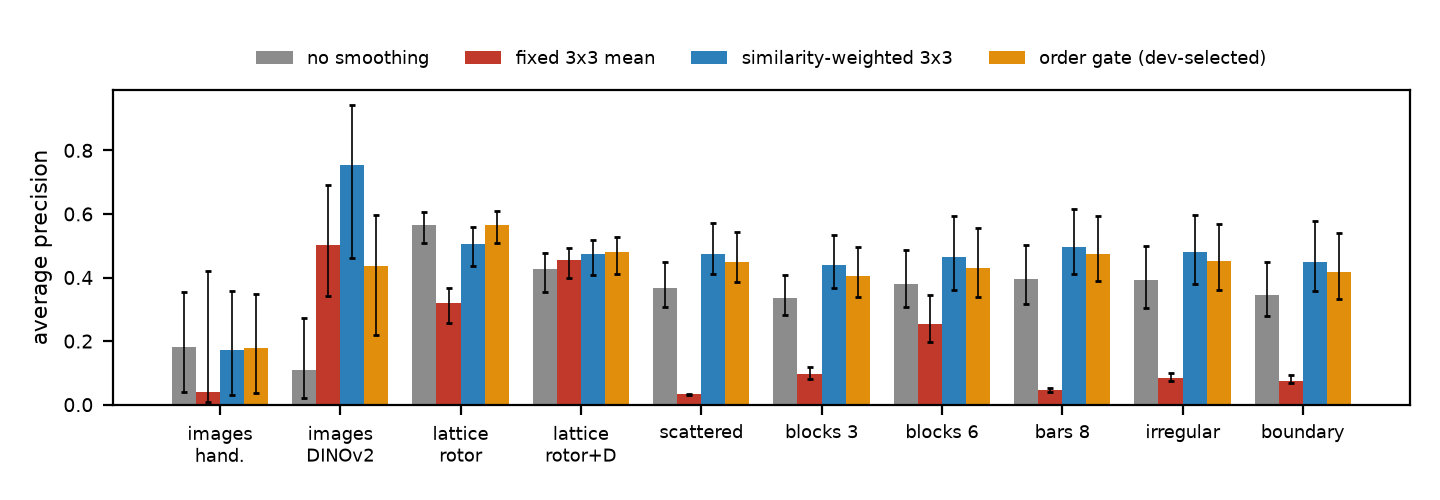
\includegraphics[width=0.9\textwidth]{fig_rules.png}
\caption{Channel A: average precision on the ten test scenarios (i)--(iii) with 95\% intervals (resampling images or simulation runs).}
\label{fig:rules}
\end{figure*}

\subsection{Channel B: arrangement anomalies}
On the three test scenarios with rearranged regions the rarity was at chance: its average precision was 0.06 (the prevalence is 0.06 to 0.07), and similarity weighting did not change that (0.06), as it must be when the distribution of the embeddings is untouched. The directional disorder reached 0.86 (95\% interval [0.84, 0.87]; paired gain over channel A [+0.78, +0.81]; Table~\ref{tab:tc}). The simple distance of a site to its eight neighbors was equally good (0.86), the isotropic disorder $D$ reached 0.57, and a local manifold statistic (the distance of a site from the plane spanned by the two leading principal directions of its $5\times5$ neighborhood) 0.48. The directional form is thus not a better detector of rearranged regions than a simple baseline; the difference lies in what else the statistics respond to. In the feature-outlier scenarios (iii), whose background has walls between domains, channel B alone found thin anomalies (scattered sites 0.56, bars 0.68) and ignored compact blocks (0.02 and 0.02), whose interior is ordered; its tail index there was 3.5, against 20 for the neighbor distance and 39 for the isotropic disorder, which respond to every wall. On the images and the MyUncle lattices channel B alone was weak (0.03, 0.01, 0.38 and 0.35).

\begin{figure*}[t]
\centering
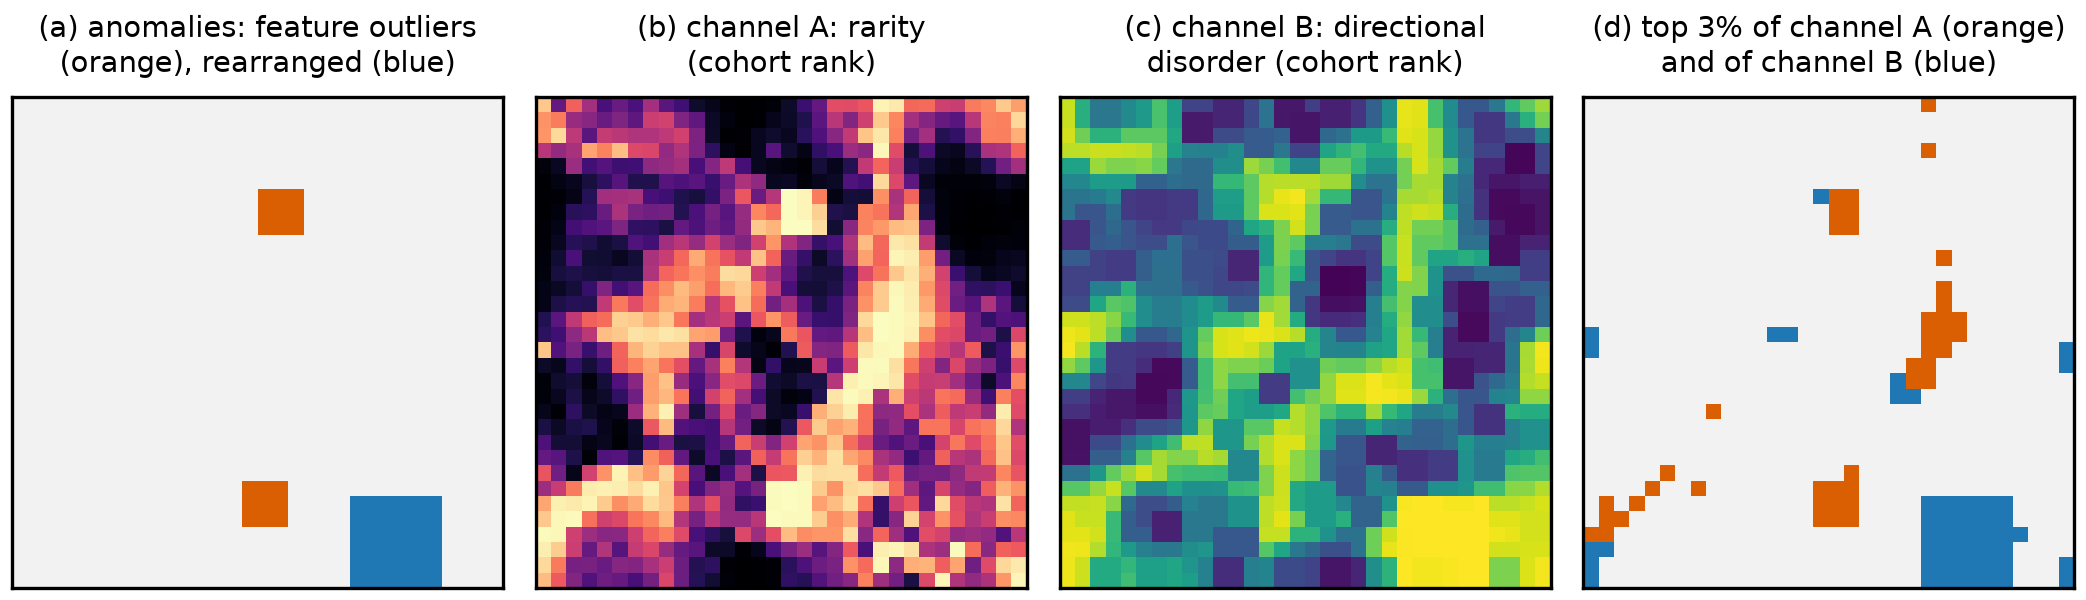
\includegraphics[width=0.92\textwidth]{fig_channels.png}
\caption{The two channels on one test lattice that contains both kinds of anomaly. Rarity marks the feature outliers and is blind to the rearranged block; the directional disorder marks the rearranged block and is blind to the compact outliers.}
\label{fig:channels}
\end{figure*}

\begin{table}[t]
\caption{Two channels on the fifteen test scenarios: mean average precision over the ten scenarios (i)--(iii), the three arrangement scenarios (iv) and the two mixed scenarios (v), and the lower-tail fitness $F$ over all fifteen with its 95\% interval.}
\label{tab:tc}
\centering\footnotesize\setlength{\tabcolsep}{2.5pt}
\begin{tabular}{lcccc}
\toprule
Detector & (i)--(iii) & (iv) & (v) & $F$ [95\% interval]\\
\midrule
Rarity, no smoothing & 0.35 & 0.06 & 0.23 & 0.16 [0.15, 0.18] \\
Rarity, fixed $3\times3$ mean & 0.19 & 0.06 & 0.07 & 0.09 [0.08, 0.11] \\
Channel A (similarity-weighted rarity) & 0.47 & 0.06 & 0.15 & 0.20 [0.19, 0.21] \\
Isotropic disorder $D$ & 0.11 & 0.57 & 0.29 & 0.12 [0.11, 0.12] \\
Local manifold statistic & 0.18 & 0.48 & 0.26 & 0.13 [0.12, 0.13] \\
Distance to the 8 neighbors & 0.20 & 0.86 & 0.53 & 0.19 [0.19, 0.19] \\
Channel B (directional disorder) & 0.24 & 0.86 & 0.49 & 0.20 [0.20, 0.21] \\
\midrule
Channel chosen by tail index & 0.47 & 0.86 & 0.49 & 0.36 [0.29, 0.46] \\
\bottomrule
\end{tabular}
\end{table}

\subsection{Label-free choice of the channel}
On the development scenarios the cohort-level selection had the highest fitness of the seven fusion rules ($F=$ 0.42, against 0.22 for channel A). On the fifteen test scenarios it reached $F=$ 0.36 (95\% interval [0.29, 0.46]), against 0.20 for channel A, 0.16 for the unsmoothed rarity and 0.09 for the fixed mean; the paired gain over channel A was +0.16 [+0.10, +0.25] and over the unsmoothed rarity +0.20 [+0.14, +0.28]. The gain came from the scenarios with rearranged regions, and nothing was lost on the ten earlier scenarios (mean AP 0.47 against 0.47; paired difference [0.00, +0.01]). The tail index chose channel A in 33 of the 34 test cohorts that contain only feature anomalies (the exception was one cohort of bars, where both channels work) and channel B in all 25 cohorts with rearranged regions; the requirement $T_B>2\times1.88$ was never the deciding condition. The directional form mattered for the choice: with the neighbor distance in place of $B_i$ the selection reached $F=$ 0.34 (paired difference to the directional version +0.02 [+0.01, +0.09]), because the walls of the block scenarios gave it a heavy tail and it was chosen wrongly there (AP 0.21 and 0.23 for $3\times3$ and boundary blocks, against 0.44 and 0.44), and with the isotropic disorder $F=$ 0.17 (+0.19 [+0.12, +0.28]). The site-wise rules were below the selection: the maximum of the standardized scores 0.25 (it failed on the DINOv2 images, 0.01), the maximum of the ranks 0.26, and the tail-weighted maxima 0.34.

Three limits were measured. (a) A cohort-level choice follows one channel. In the mixed cohorts it chose channel B and reached an AP of 0.45 and 0.53 over both kinds of anomaly (channel A: 0.20 and 0.09), but taken by kind, the rearranged sites were found by channel B (0.62 and 0.62) and the feature outliers only by the rarity (0.52 and 0.49 unsmoothed; channel B 0.02 and 0.05): when both kinds occur together, the two maps must be read side by side (Fig.~\ref{fig:channels}). (b) In the smooth background of the mixed cohorts similarity weighting lowered the AP of scattered feature outliers from 0.49 to 0.08, because coherent patches of mildly rare normal sites are reinforced; channel A is not uniformly better than the unsmoothed rarity. (c) A first attempt, fixed blends of the ranks of channel A and of the isotropic disorder, had been selected on thirteen of the development scenarios ($F=$ 0.256 against 0.238) and did not beat channel A on the corresponding test scenarios (0.206 against 0.214); the directional statistic and the tail index were designed after that, so thirteen of the fifteen test scenarios had been used once before.

\subsection{What did not help}
\label{sec:neg}
\emph{Order gates.} The development-selected gates did not beat ordinary similarity on the ten test scenarios: the gate on compatibility reached $F=$ 0.30 and the gates on the resultant length and on $H_\chi$ 0.31, against 0.32 for the untuned similarity-weighted rule ($-$0.02 [$-$0.04, 0.00] and $-$0.02 [$-$0.03, 0.00]); the last two gave the same scores to within 0.01, as the monotone relation of $H_\chi$ and $R_i$ requires. Local order was useful as a channel of its own, not as a gate on the rarity, and the $d$-dimensional entropy is reported as a formal result. \emph{Other rules.} The one-sided rule matched no smoothing (0.00 [0.00, +0.01] in $F$), and so did the nucleation-and-growth rule ($F=$ 0.23; 0.00 [0.00, 0.00]; $-$0.09 [$-$0.19, $-$0.04] against similarity weighting). The retention of the top-3\% sites under the fixed mean correlated with the effect of the fixed mean over 68 cohorts (Spearman $\rho=$ 0.43, $p=$ 0.0002), but a choice between the fixed mean and no smoothing based on it reached a mean AP of 0.36 on the test cohorts against 0.37 for no smoothing and 0.48 for similarity weighting. \emph{Search.} Among the 460 rule configurations the frozen fixed mean ranked 455th on the development fitness (0.13; optimum 0.41). With 40 evaluations and 100 repetitions, random search found a configuration in the top 5\% in 94\% of the runs, the GaaR strategies in 70\% (greedy), 81\% (restart) and 80\% (population), and in the top 1\% in 67\% against 53\%, 58\% and 59\%: GaaR was not better than random search here, because many configurations of the similarity-weighted family are nearly equivalent, and its champion ($F=$ 0.31) was no better than the untuned rule. An earlier search of the scoring configuration itself (360 configurations; repository) gave a gain on fresh scenarios of +0.08 with a 95\% interval of [$-$0.05, +0.17], which includes zero.

\begin{figure}[t]
\centering
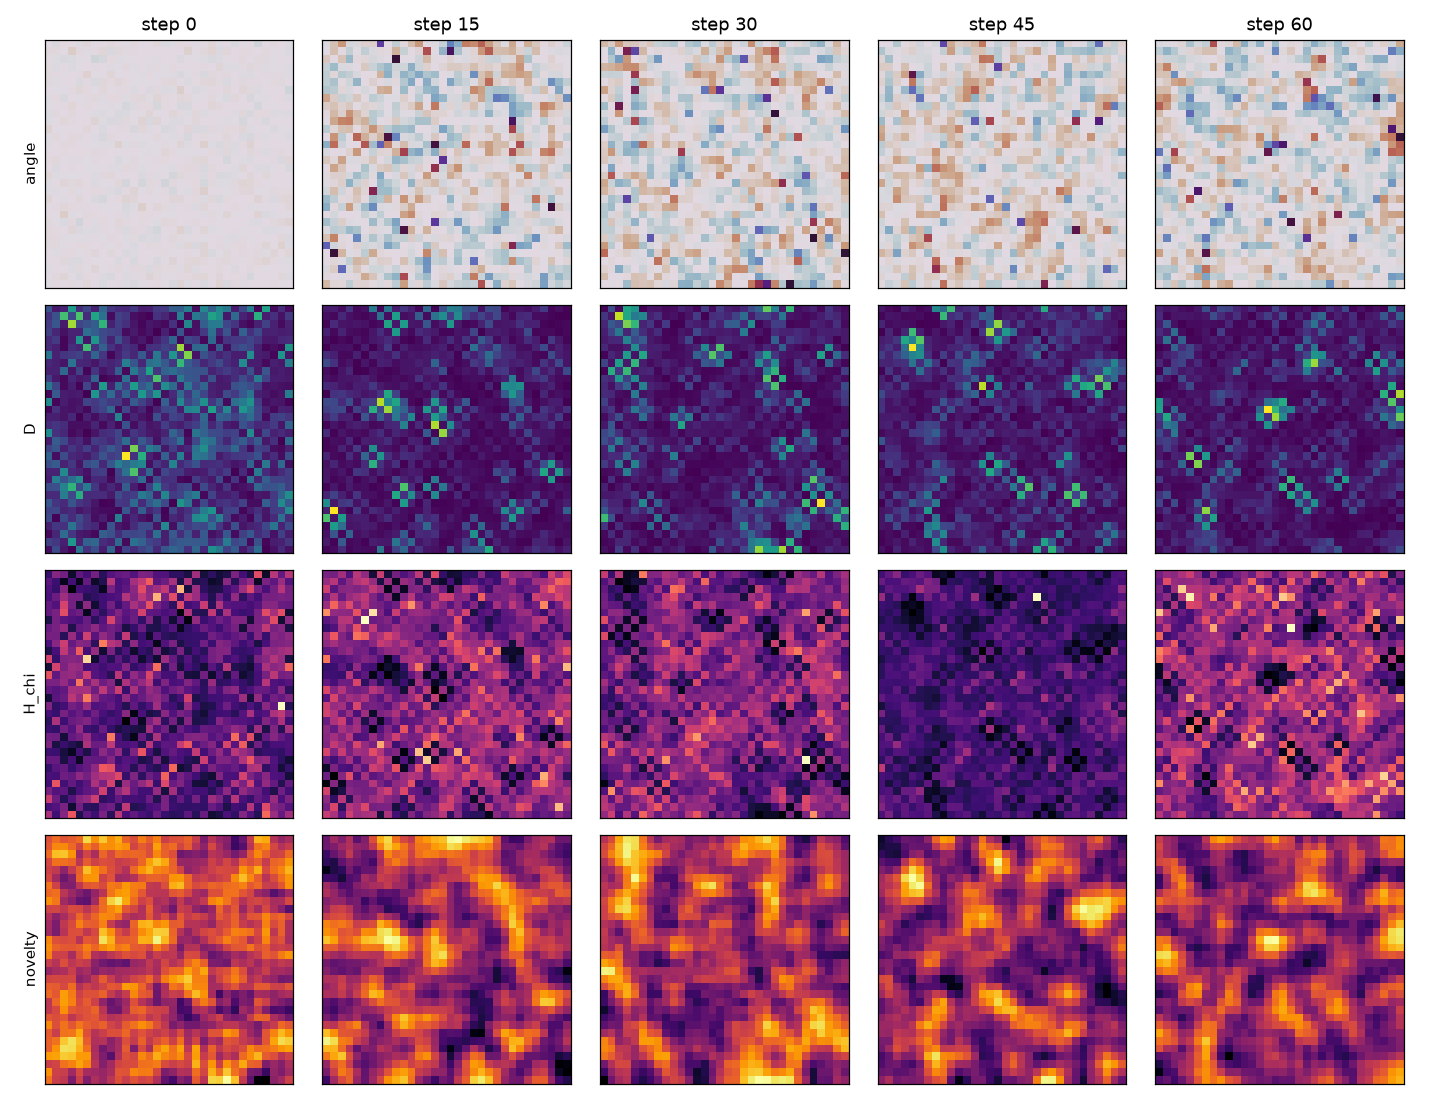
\includegraphics[width=0.95\columnwidth]{fig_bridge_maps.png}
\caption{A MyUncle simulation analyzed with MyUncleVision (chiral scaffold preset, $32\times32$ sites). Rows: rotor angle, local disorder $D$, order information $H_\chi$ ($d=2$) and the earlier frozen novelty score (rarity, fixed $3\times3$ mean); columns: steps 0, 15, 30, 45 and 60.}
\label{fig:maps}
\end{figure}

\section{Limitations and future work}
The lattices and the images are simulated and were written by the author of the method (the simulation is MyUncle's and its parameter sets are not fitted to measurements; the generators have Gaussian noise, and a permutation is an idealized arrangement anomaly that changes nothing but the arrangement); nothing here shows that the method finds anything in an experimental system. Development and test data come from the same generator families, 16 to 50 independent units per test scenario are few, and the choice among rules uses development labels. The tail index compares two numbers per cohort: it cannot serve a cohort that contains both kinds of anomaly, and when neither channel has a tail (the DINOv2 images, 2.1 against 1.7) the choice rests on the default. Channel B needs a background that is locally ordered; where normal sites are themselves disordered it has nothing to measure. Novelty is not a defect: a rare or disorganized state may be a rare preparation or a known feature that is merely uncommon. The rarity score was compared with other detectors (isolation forest, local outlier factor, nearest-neighbor and Mahalanobis distance) under the earlier fixed smoothing (repository): a smoothed Mahalanobis baseline scored higher on the development images, so the rarity is not claimed to be the best channel-A detector. Planned: validation on public data with logical anomalies \citep{Bergmann2022} and on experimental micrographs with independently established defects, blinded expert review, more units per scenario, a site-wise fusion that serves mixed cohorts, and other filters of the bilateral and non-local-means families as baselines.

\section{Conclusions}
Rarity and local order are complementary label-free channels on a lattice of embeddings. Rarity, aggregated with similarity weights instead of a fixed window, finds what is unusual; the directional local disorder, a quantity of the MyUncle lattice model, finds ordinary embeddings in the wrong arrangement, to which rarity is blind (average precision 0.06 against 0.86). A label-free tail index chose channel A in the test cohorts with feature anomalies and channel B in those with rearranged regions, and raised the lower-tail average precision over fifteen independent test scenarios from 0.20 to 0.36 (paired interval of the gain +0.10 to +0.25) without loss on the scenarios that contain only feature anomalies. Cohorts with both kinds of anomaly still need both maps, and all evidence is simulated; experimental validation is the next step.

\section*{Declarations}
\small
\textbf{Funding:} no external funding. \textbf{Competing interests:} the author declares no competing interests. \textbf{CRediT:} Leon Sandler, sole author: conceptualization, methodology, software, validation, formal analysis, investigation, visualization, writing -- original draft, writing -- review and editing. \textbf{Data and code availability:} code, tests, benchmarks, search tables, seeds and results are open at \url{https://github.com/sandlerleon/MyUncleVision} (MIT license; vendored MyUncle and GaaR cores unmodified, GaaR commit 4021e64) and archived at \url{https://doi.org/10.5281/zenodo.24066260} (all versions). No experimental, patient or tissue data were used. \textbf{Generative AI:} during the preparation of this work the author used Claude (Anthropic) to assist with writing and testing the code, running the analyses and drafting the text and figures; the author reviewed and edited the content and takes full responsibility for it.
\normalsize

\begin{thebibliography}{}
\footnotesize
\bibitem[{Banerjee et~al.(2005)}]{Banerjee2005} Banerjee, A., Dhillon, I.S., Ghosh, J., Sra, S., 2005. Clustering on the unit hypersphere using von Mises-Fisher distributions. J. Mach. Learn. Res. 6, 1345--1382.
\bibitem[{Baron and Poznanski(2017)}]{Baron2017} Baron, D., Poznanski, D., 2017. The weirdest SDSS galaxies: results from an outlier detection algorithm. Mon. Not. R. Astron. Soc. 465, 4530--4555. \url{https://doi.org/10.1093/mnras/stw3021}.
\bibitem[{Bergmann et~al.(2022)}]{Bergmann2022} Bergmann, P., Batzner, K., Fauser, M., Sattlegger, D., Steger, C., 2022. Beyond dents and scratches: logical constraints in unsupervised anomaly detection and localization. Int. J. Comput. Vis. 130, 947--969. \url{https://doi.org/10.1007/s11263-022-01578-9}.
\bibitem[{Canny(1986)}]{Canny1986} Canny, J., 1986. A computational approach to edge detection. IEEE Trans. Pattern Anal. Mach. Intell. 8, 679--698. \url{https://doi.org/10.1109/TPAMI.1986.4767851}.
\bibitem[{Chandola et~al.(2009)}]{Chandola2009} Chandola, V., Banerjee, A., Kumar, V., 2009. Anomaly detection: a survey. ACM Comput. Surv. 41 (3), 15. \url{https://doi.org/10.1145/1541880.1541882}.
\bibitem[{Kuwahara et~al.(1976)}]{Kuwahara1976} Kuwahara, M., Hachimura, K., Eiho, S., Kinoshita, M., 1976. Processing of RI-angiocardiographic images, in: Preston, K., Onoe, M. (Eds.), Digital Processing of Biomedical Images. Plenum Press, New York, pp. 187--202.
\bibitem[{Lochner and Bassett(2021)}]{Lochner2021} Lochner, M., Bassett, B.A., 2021. Astronomaly: personalised active anomaly detection in astronomical data. Astron. Comput. 36, 100481. \url{https://doi.org/10.1016/j.ascom.2021.100481}.
\bibitem[{Mardia and Jupp(2000)}]{Mardia2000} Mardia, K.V., Jupp, P.E., 2000. Directional Statistics. Wiley, Chichester.
\bibitem[{Oquab et~al.(2023)}]{Oquab2023} Oquab, M., Darcet, T., Moutakanni, T., et al., 2023. DINOv2: learning robust visual features without supervision. arXiv:2304.07193. \url{https://doi.org/10.48550/arXiv.2304.07193}.
\bibitem[{Pedregosa et~al.(2011)}]{Pedregosa2011} Pedregosa, F., Varoquaux, G., Gramfort, A., et al., 2011. Scikit-learn: machine learning in Python. J. Mach. Learn. Res. 12, 2825--2830.
\bibitem[{Roth et~al.(2022)}]{Roth2022} Roth, K., Pemula, L., Zepeda, J., Sch{\"o}lkopf, B., Brox, T., Gehler, P., 2022. Towards total recall in industrial anomaly detection, in: Proc. IEEE/CVF Conf. Comput. Vis. Pattern Recognit. (CVPR), pp. 14318--14328.
\bibitem[{Rousseeuw and Croux(1993)}]{Rousseeuw1993} Rousseeuw, P.J., Croux, C., 1993. Alternatives to the median absolute deviation. J. Am. Stat. Assoc. 88, 1273--1283. \url{https://doi.org/10.1080/01621459.1993.10476408}.
\bibitem[{Ruifrok and Johnston(2001)}]{Ruifrok2001} Ruifrok, A.C., Johnston, D.A., 2001. Quantification of histochemical staining by color deconvolution. Anal. Quant. Cytol. Histol. 23, 291--299.
\bibitem[{Sandler(2026a)}]{MyUncle2026} Sandler, L., 2026a. MyUncle: a compact maintenance-lattice framework (software). Zenodo. \url{https://doi.org/10.5281/zenodo.21223570}.
\bibitem[{Sandler(2026c)}]{GaaR2026} Sandler, L., 2026c. GaaR: goal-aware adaptive regulation, evolutionary search on consumer hardware (software). GitHub, commit 4021e64. \url{https://github.com/sandlerleon/GaaR}.
\bibitem[{Sandler(2026b)}]{MyUncleVision2026} Sandler, L., 2026b. MyUncleVision: a lattice-based framework for unsupervised anomaly discovery in images (software). Zenodo. \url{https://doi.org/10.5281/zenodo.24066260}.
\bibitem[{Schlegl et~al.(2019)}]{Schlegl2019} Schlegl, T., Seeb{\"o}ck, P., Waldstein, S.M., Langs, G., Schmidt-Erfurth, U., 2019. f-AnoGAN: fast unsupervised anomaly detection with generative adversarial networks. Med. Image Anal. 54, 30--44. \url{https://doi.org/10.1016/j.media.2019.01.010}.
\end{thebibliography}

\end{document}
